\documentclass[8pt,aspectratio=169]{beamer}
\usepackage[utf8]{inputenc}
\usepackage{graphicx}
\usepackage{amsmath,amssymb}
\usepackage{listings}
\usepackage{xcolor}
\usepackage{tikz}
\usepackage{tcolorbox}

\usetheme{Madrid}
\setbeamertemplate{navigation symbols}{}

% Template colors (lavender scheme matching Week 3)
\definecolor{mlblue}{RGB}{0,102,204}
\definecolor{mlpurple}{RGB}{51,51,178}
\definecolor{mllavender}{RGB}{173,173,224}
\definecolor{mllavender2}{RGB}{193,193,232}
\definecolor{mllavender3}{RGB}{204,204,235}
\definecolor{mllavender4}{RGB}{214,214,239}
\definecolor{mlorange}{RGB}{255,127,14}
\definecolor{mlgreen}{RGB}{44,160,44}
\definecolor{mlred}{RGB}{214,39,40}

% Apply custom colors to Madrid theme
\setbeamercolor{palette primary}{bg=mllavender3,fg=mlpurple}
\setbeamercolor{palette secondary}{bg=mllavender2,fg=mlpurple}
\setbeamercolor{palette tertiary}{bg=mllavender,fg=white}
\setbeamercolor{palette quaternary}{bg=mlpurple,fg=white}
\setbeamercolor{structure}{fg=mlpurple}
\setbeamercolor{frametitle}{fg=mlpurple,bg=mllavender3}

% Legacy color compatibility
\definecolor{darkblue}{RGB}{0,51,102}
\definecolor{lightblue}{RGB}{173,216,230}
\definecolor{codegreen}{RGB}{0,128,0}
\definecolor{codegray}{RGB}{150,150,150}
\definecolor{backcolor}{RGB}{245,245,245}

\lstset{
    backgroundcolor=\color{backcolor},
    basicstyle=\ttfamily\tiny,
    breaklines=true,
    language=Python
}

\newcommand{\given}{\mid}
\newcommand{\highlight}[1]{\textcolor{mlred}{\textbf{#1}}}
\newcommand{\eqbox}[1]{\begin{tcolorbox}[colback=blue!5!white,colframe=blue!75!black]#1\end{tcolorbox}}

% BSc Pedagogical boxes (matching Week 3)
\newtcolorbox{checkpoint}[1][]{
    colback=yellow!10!white,
    colframe=yellow!75!black,
    title=\textbf{Checkpoint: #1},
    fonttitle=\bfseries,
    left=3pt, right=3pt, top=3pt, bottom=3pt
}

\newtcolorbox{intuition}[1][]{
    colback=purple!5!white,
    colframe=purple!75!black,
    title=\textbf{Intuition: #1},
    fonttitle=\bfseries,
    left=3pt, right=3pt, top=3pt, bottom=3pt
}

\newtcolorbox{realworld}[1][]{
    colback=orange!5!white,
    colframe=orange!75!black,
    title=\textbf{Real World: #1},
    fonttitle=\bfseries,
    left=3pt, right=3pt, top=3pt, bottom=3pt
}

% Bottom annotation command
\newcommand{\bottomnote}[1]{%
\vfill
\vspace{-2mm}
\textcolor{mllavender2}{\rule{\textwidth}{0.4pt}}
\vspace{1mm}
\footnotesize
\textbf{#1}
}

\title[Week 4: Seq2Seq]{Natural Language Processing}
\subtitle{Week 4: The Compression Journey}
\institute{From Meaning to Numbers and Back Again}
\author{}
\date{}

\begin{document}

\begin{frame}[plain]
    \titlepage
\end{frame}

% Discovery-based opening
\begin{frame}{Before We Begin: A Thought Experiment}
    \begin{center}
    \textbf{\Large Imagine You're Designing a Translation System}
    \end{center}

    \vspace{1em}
    \begin{columns}[T]
        \begin{column}{0.55\textwidth}
            \textbf{Your Challenge:}

            Translate this 40-word sentence into French:

            \vspace{0.5em}
            \textit{\small ``The International Conference on Machine Learning, which is one of the premier venues for presenting research in machine learning and attracts submissions from researchers around the world, accepted our paper.''}

            \vspace{1em}
            \textbf{Design Constraints:}
            \begin{enumerate}
                \item You can only write down 256 numbers total
                \item These numbers must capture ALL the meaning
                \item Then translate from just those 256 numbers
                \item You cannot look back at the original!
            \end{enumerate}

            \vspace{1em}
            \colorbox{orange!10}{\parbox{0.95\columnwidth}{
                \textbf{Question:} Can 256 numbers really hold 40 words of meaning? What happens to:
                \begin{itemize}
                    \item ``International'' (important detail)
                    \item ``premier venues'' (significance)
                    \item ``researchers around the world'' (scale)
                \end{itemize}
            }}
        \end{column}

        \begin{column}{0.43\textwidth}
            \textbf{Your Design:}

            \vspace{0.5em}
            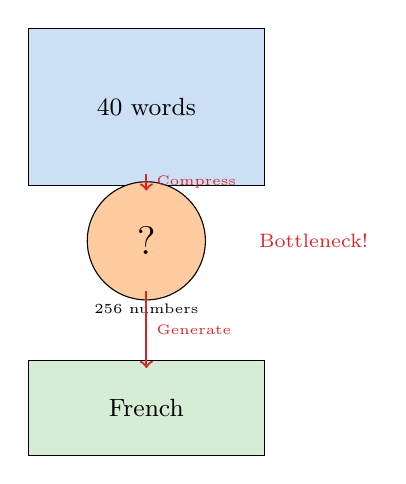
\begin{tikzpicture}[scale=0.85, every node/.style={font=\small}]
                % Input text box
                \node[draw, rectangle, minimum width=3cm, minimum height=2cm, fill=mlblue!20] at (0, 2) {40 words};

                % Compression bottleneck
                \node[draw, circle, fill=mlorange!40, minimum size=1.5cm] at (0, 0) {\Large ?};
                \node[below, font=\tiny] at (0, -0.8) {256 numbers};

                % Output
                \node[draw, rectangle, minimum width=3cm, minimum height=1.2cm, fill=mlgreen!20] at (0, -2.5) {French};

                % Arrows
                \draw[->, thick, mlred] (0, 1) -- (0, 0.75) node[midway, right, font=\tiny] {Compress};
                \draw[->, thick, mlred] (0, -0.75) -- (0, -1.9) node[midway, right, font=\tiny] {Generate};

                % Warning annotation
                \node[mlred, font=\scriptsize] at (2.5, 0) {Bottleneck!};
            \end{tikzpicture}

            \vspace{1em}
            \textbf{Think about it:}
            \begin{itemize}
                \item What information survives?
                \item What gets lost?
                \item Is there a better way?
            \end{itemize}
        \end{column}
    \end{columns}

    \bottomnote{Next slide reveals: This is exactly the problem that launched the attention revolution!}
\end{frame}

\begin{frame}{Learning Objectives}
    \textbf{By the end of this lecture, you will understand:}
    \begin{enumerate}
        \item Why we need numbers to represent words (from first principles)
        \item How compression creates an information bottleneck
        \item What ``context'' and ``hidden state'' actually mean
        \item How attention solves the compression problem
        \item Why this matters for all modern NLP
    \end{enumerate}

    \vspace{1em}
    \textbf{Prerequisites from Week 3:}
    \begin{itemize}
        \item Basic understanding that neural networks process numbers
        \item Concept of sequential processing (RNN idea)
        \item Backpropagation intuition
    \end{itemize}
\end{frame}

\begin{frame}{Table of Contents}
    \tableofcontents
\end{frame}

\section{Act 1: The Compression Challenge}

\begin{frame}[t]{The Core Problem: Computers Don't Understand Words}
    \textbf{Start with the fundamental challenge:}

    \vspace{0.5em}
    You want to translate: ``The black cat sat on the mat'' $\rightarrow$ French

    \vspace{0.5em}
    \textbf{The Computer's Dilemma:}
    \begin{itemize}
        \item Computer sees: \texttt{['T', 'h', 'e', ' ', 'b', 'l', 'a', ...]}
        \item These are just character codes (bytes)
        \item \highlight{No meaning, no relationships, no structure}
    \end{itemize}

    \vspace{0.5em}
    \begin{columns}[T]
        \column{0.5\textwidth}
        \textbf{What the computer sees:}
        \begin{itemize}
            \item ``cat'' = [99, 97, 116]
            \item ``dog'' = [100, 111, 103]
            \item ``sat'' = [115, 97, 116]
        \end{itemize}

        \column{0.5\textwidth}
        \textbf{Problem:}
        \begin{itemize}
            \item ``cat'' and ``sat'' share [97, 116]
            \item Does that mean they're similar?
            \item \textcolor{red}{No! Character overlap $\neq$ meaning}
        \end{itemize}
    \end{columns}

    \vspace{1em}
    \textbf{Key Question:} How do we give computers a ``numerical understanding'' of word meaning?
\end{frame}

\begin{frame}[t]{From Words to Numbers: The Embedding Idea}
    \textbf{The solution: Represent each word as a vector of numbers}

    \vspace{0.5em}
    \textbf{Build intuition with simple example:}

    Imagine describing animals with just 3 properties:
    \begin{itemize}
        \item Size (0=tiny, 1=huge)
        \item Cuteness (0=scary, 1=adorable)
        \item Speed (0=slow, 1=fast)
    \end{itemize}

    \vspace{0.5em}
    \begin{center}
    \begin{tabular}{|l|c|c|c|}
        \hline
        \textbf{Word} & \textbf{Size} & \textbf{Cute} & \textbf{Speed} \\
        \hline
        cat & 0.3 & 0.9 & 0.6 \\
        dog & 0.5 & 0.8 & 0.5 \\
        mouse & 0.1 & 0.7 & 0.8 \\
        elephant & 0.95 & 0.4 & 0.2 \\
        \hline
    \end{tabular}
    \end{center}

    \vspace{0.5em}
    Now computers can compute:
    \begin{itemize}
        \item Similarity: cat $\approx$ dog (vectors are close)
        \item Difference: cat $\neq$ elephant (vectors are far)
        \item \highlight{This is called a ``word embedding''}
    \end{itemize}

    \vspace{0.5em}
    \textbf{Reality:} We use 100-300 dimensions (not just 3), learned from data

    \vspace{1em}
    \begin{checkpoint}[Understanding Embeddings]
    \textbf{Quick Check:} Why do we need embeddings?

    \vspace{0.3em}
    \textbf{Answer:} Computers only process numbers. Embeddings give words numerical meaning so similar words have similar vectors (cat ≈ dog in vector space).
    \end{checkpoint}
\end{frame}

\begin{frame}[t]{What is a ``Hidden State''? Building Intuition}
    \textbf{Now we have numbers for words. Next problem: Understanding sentences}

    \vspace{0.5em}
    \textbf{Human analogy - Reading comprehension:}

    As you read ``The black cat sat on the mat'':
    \begin{enumerate}
        \item After ``The'' $\rightarrow$ You know: article, something coming
        \item After ``The black'' $\rightarrow$ You know: a dark-colored thing
        \item After ``The black cat'' $\rightarrow$ You know: a specific animal
        \item After full sentence $\rightarrow$ You know: complete scene
    \end{enumerate}

    \vspace{0.5em}
    \textbf{Your ``understanding'' evolves as you read!}

    \vspace{1em}
    \textbf{Neural network equivalent:}
    \begin{itemize}
        \item Network maintains a vector that represents ``current understanding''
        \item This vector updates with each new word
        \item \highlight{This evolving vector is called the ``hidden state''}
        \item Final hidden state = complete understanding of sentence
    \end{itemize}

    \vspace{0.5em}
    \textbf{Technical name:} When we update understanding word-by-word, we call this a ``Recurrent Neural Network'' (RNN from Week 3)
\end{frame}

\begin{frame}[t]{The Compression Problem Emerges}
    \textbf{Now the real challenge appears:}

    \vspace{0.5em}
    We need to translate: ``The black cat sat on the mat'' $\rightarrow$ ``Le chat noir s'est assis sur le tapis''

    \vspace{0.5em}
    \textbf{Two-stage process (like human translation):}

    \begin{center}
    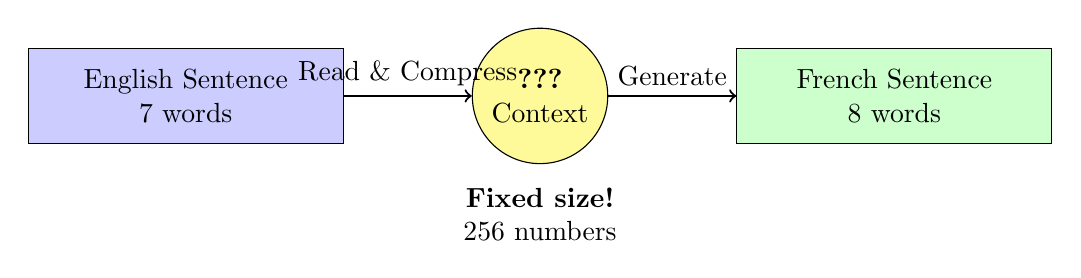
\begin{tikzpicture}[scale=0.9]
        \node[draw, rectangle, minimum width=4cm, minimum height=1.2cm, fill=blue!20, align=center] (input) at (0,0) {English Sentence\\7 words};

        \node[draw, circle, fill=yellow!40, minimum size=1.5cm, align=center] (compressed) at (5,0) {\textbf{???}\\Context};

        \node[draw, rectangle, minimum width=4cm, minimum height=1.2cm, fill=green!20, align=center] (output) at (10,0) {French Sentence\\8 words};

        \draw[->, thick] (input) -- (compressed) node[midway, above] {Read \& Compress};
        \draw[->, thick] (compressed) -- (output) node[midway, above] {Generate};

        \node[below of=compressed, node distance=1.5cm, align=center] {\textbf{Fixed size!}\\256 numbers};
    \end{tikzpicture}
    \end{center}

    \vspace{0.5em}
    \textbf{The bottleneck:}
    \begin{itemize}
        \item 7 words of meaning $\rightarrow$ compressed to 256 numbers
        \item Then generate 8 words from just those 256 numbers
        \item \highlight{Can 256 numbers hold all the information?}
    \end{itemize}

    \vspace{0.5em}
    \textbf{Key Question:} What happens with longer sentences? 100 words $\rightarrow$ still 256 numbers?
\end{frame}

\begin{frame}[t]{Quantifying the Compression Problem}
    \textbf{Let's calculate how much compression we're doing:}

    \vspace{0.5em}
    \textbf{Information content (rough estimate):}
    \begin{itemize}
        \item Each word embedding: 100 dimensions (numbers)
        \item 7-word sentence: $7 \times 100 = 700$ numbers of information
        \item Context vector: \textbf{only 256 numbers}
        \item \highlight{Compression ratio: 700:256 $\approx$ 2.7:1}
    \end{itemize}

    \vspace{0.5em}
    \textbf{What about longer sentences?}

    \begin{center}
    \begin{tabular}{|l|c|c|c|c|}
        \hline
        \textbf{Length} & \textbf{Input Dims} & \textbf{Context Dims} & \textbf{Ratio} & \textbf{Quality} \\
        \hline
        5 words & 500 & 256 & 2:1 & Good \\
        20 words & 2000 & 256 & 8:1 & Mediocre \\
        50 words & 5000 & 256 & 20:1 & Poor \\
        100 words & 10000 & 256 & 40:1 & Very Poor \\
        \hline
    \end{tabular}
    \end{center}

    \vspace{0.5em}
    \begin{tcolorbox}[colback=red!10!white,colframe=red!75!black]
    \textbf{The Information Bottleneck:} Longer sentences lose more information!

    Like trying to fit a whole book into a single paragraph - something must be lost.
    \end{tcolorbox}

    \vspace{0.5em}
    \textbf{Next question:} Can we avoid this bottleneck? (Spoiler: Yes, with attention!)
\end{frame}

\section{Act 2: The Encoder-Decoder Solution (And Its Limits)}

\begin{frame}[t]{The Two-Network Architecture}
    \textbf{The key insight: Separate ``reading'' from ``writing''}

    \vspace{0.5em}
    \textbf{Why two networks? Build from human behavior:}

    When YOU translate:
    \begin{enumerate}
        \item \textbf{Phase 1 (Reading):} Read and understand the English sentence
        \begin{itemize}
            \item Process word-by-word
            \item Build complete understanding
            \item Store meaning in your memory
        \end{itemize}
        \item \textbf{Phase 2 (Writing):} Generate the French translation
        \begin{itemize}
            \item Start from your understanding
            \item Generate word-by-word in French
            \item Use grammar and vocabulary of target language
        \end{itemize}
    \end{enumerate}

    \vspace{0.5em}
    \textbf{Neural equivalent:}
    \begin{itemize}
        \item \textbf{Encoder network:} Reads input, builds ``hidden state'' (understanding)
        \item \textbf{Context vector:} Final hidden state (compressed meaning)
        \item \textbf{Decoder network:} Generates output from context
    \end{itemize}

    \vspace{0.5em}
    \textbf{Technical names you now understand:}
    \begin{itemize}
        \item ``Sequence-to-Sequence'' (Seq2Seq) = this two-network setup
        \item ``Encoder-Decoder architecture'' = same thing
    \end{itemize}

    \vspace{1em}
    \begin{intuition}[Why Two Networks?]
    Just like human translation: FIRST fully understand the source sentence (encoder), THEN generate the target (decoder). Mixing these would be confusing - like trying to speak French while still reading English!
    \end{intuition}
\end{frame}

\begin{frame}[fragile,t]{Encoder: Building Understanding Step-by-Step}
    \textbf{Concrete example: Encoding ``The cat sat''}

    \vspace{0.5em}
    \begin{columns}[T]
        \column{0.55\textwidth}
        \textbf{Step-by-step processing:}

        \textbf{Step 1: Read ``The''}
        \begin{itemize}
            \item Convert to embedding: [0.2, 0.5, -0.1, ...] (100d)
            \item Initial understanding: $h_0$ = [0, 0, 0, ...] (256d)
            \item Update: $h_1$ = RNN(``The'', $h_0$)
            \item New understanding: [0.1, -0.05, 0.03, ...] (256d)
        \end{itemize}

        \textbf{Step 2: Read ``cat''}
        \begin{itemize}
            \item Embedding: [0.7, -0.3, 0.4, ...] (100d)
            \item Previous understanding: $h_1$
            \item Update: $h_2$ = RNN(``cat'', $h_1$)
            \item New understanding: [0.3, 0.2, -0.1, ...] (256d)
        \end{itemize}

        \textbf{Step 3: Read ``sat''}
        \begin{itemize}
            \item Embedding: [-0.2, 0.6, 0.1, ...]
            \item Update: $h_3$ = RNN(``sat'', $h_2$)
            \item \highlight{Final understanding: $h_3$ = context vector}
        \end{itemize}

        \column{0.43\textwidth}
        \begin{center}
        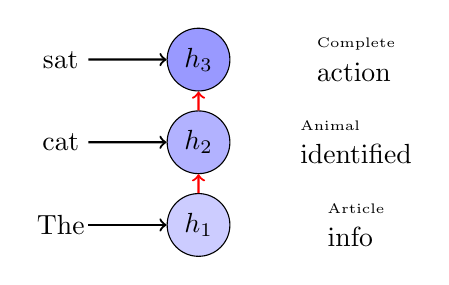
\begin{tikzpicture}[scale=0.7]
            \node at (0,0) {The};
            \node at (0,1.5) {cat};
            \node at (0,3) {sat};

            \node[draw, circle, fill=blue!20] (h1) at (2.5,0) {$h_1$};
            \node[draw, circle, fill=blue!30] (h2) at (2.5,1.5) {$h_2$};
            \node[draw, circle, fill=blue!40] (h3) at (2.5,3) {$h_3$};

            \draw[->, thick] (0.5,0) -- (h1);
            \draw[->, thick] (0.5,1.5) -- (h2);
            \draw[->, thick] (0.5,3) -- (h3);

            \draw[->, thick, red] (h1) -- (h2);
            \draw[->, thick, red] (h2) -- (h3);

            \node[right of=h1, node distance=2cm, align=left] {\tiny Article\\info};
            \node[right of=h2, node distance=2cm, align=left] {\tiny Animal\\identified};
            \node[right of=h3, node distance=2cm, align=left] {\tiny Complete\\action};
        \end{tikzpicture}
        \end{center}

        \vspace{1em}
        \textbf{Key insight:}
        \begin{itemize}
            \item Each $h_t$ = accumulated understanding
            \item Always 256 dimensions
            \item Final $h_3$ goes to decoder
        \end{itemize}
    \end{columns}
\end{frame}

\begin{frame}[fragile,t]{Decoder: Generating from Understanding}
    \textbf{Now generate French from the context vector}

    \vspace{0.5em}
    \begin{columns}[T]
        \column{0.55\textwidth}
        \textbf{Generation process:}

        \textbf{Step 0: Start}
        \begin{itemize}
            \item Input: <START> token
            \item Context: $c = h_3$ from encoder (256d)
            \item Generate: $s_0$ = RNN(<START>, $c$)
            \item Predict probabilities: P(``Le'') = 0.6, P(``Un'') = 0.3, ...
            \item \highlight{Choose ``Le''}
        \end{itemize}

        \textbf{Step 1: Continue}
        \begin{itemize}
            \item Input: ``Le'' (what we just generated)
            \item Context: still $c$ (same context!)
            \item Generate: $s_1$ = RNN(``Le'', $s_0$, $c$)
            \item Predict: P(``chat'') = 0.7, P(``chien'') = 0.2, ...
            \item \highlight{Choose ``chat''}
        \end{itemize}

        \textbf{Step 2: Continue until <END>}
        \begin{itemize}
            \item Input: ``chat''
            \item Generate: $s_2$ = RNN(``chat'', $s_1$, $c$)
            \item Keep going until model outputs <END>
        \end{itemize}

        \column{0.43\textwidth}
        \begin{center}
        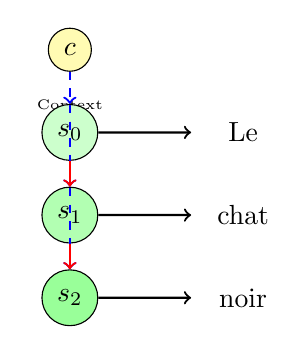
\begin{tikzpicture}[scale=0.7]
            \node[draw, circle, fill=yellow!30] (context) at (0,4) {$c$};
            \node[below of=context, node distance=0.7cm] {\tiny Context};

            \node[draw, circle, fill=green!20] (s0) at (0,2.5) {$s_0$};
            \node[draw, circle, fill=green!30] (s1) at (0,1) {$s_1$};
            \node[draw, circle, fill=green!40] (s2) at (0,-0.5) {$s_2$};

            \node[right of=s0, node distance=2.2cm] {Le};
            \node[right of=s1, node distance=2.2cm] {chat};
            \node[right of=s2, node distance=2.2cm] {noir};

            \draw[->, thick, blue, dashed] (context) -- (s0);
            \draw[->, thick, blue, dashed] (context) -- (s1);
            \draw[->, thick, blue, dashed] (context) -- (s2);

            \draw[->, thick, red] (s0) -- (s1);
            \draw[->, thick, red] (s1) -- (s2);

            \draw[->, thick] (s0) -- (2.2,2.5);
            \draw[->, thick] (s1) -- (2.2,1);
            \draw[->, thick] (s2) -- (2.2,-0.5);
        \end{tikzpicture}
        \end{center}

        \vspace{0.5em}
        \textbf{Key observations:}
        \begin{itemize}
            \item Context $c$ used at every step
            \item Previous word fed back in
            \item Generate one word at a time
            \item Stop when <END> predicted
        \end{itemize}
    \end{columns}
\end{frame}

\begin{frame}[t]{The First Success: Short Sentences Work Great!}
    \textbf{Initial results (5-10 word sentences):}

    \vspace{0.5em}
    \begin{center}
    \begin{tabular}{|l|l|l|}
        \hline
        \textbf{English} & \textbf{French Translation} & \textbf{Result} \\
        \hline
        The cat sat & Le chat s'est assis & \textcolor{green}{Perfect!} \\
        I love you & Je t'aime & \textcolor{green}{Perfect!} \\
        Hello world & Bonjour le monde & \textcolor{green}{Perfect!} \\
        Good morning & Bonjour & \textcolor{green}{Perfect!} \\
        See you later & A plus tard & \textcolor{green}{Perfect!} \\
        \hline
    \end{tabular}
    \end{center}

    \vspace{0.5em}
    \textbf{Performance on short sentences:}
    \begin{itemize}
        \item 5-10 words: \textbf{BLEU 35.2} (excellent quality)
        \item Captures meaning correctly
        \item Word order appropriate
        \item Grammar correct
    \end{itemize}

    \vspace{0.5em}
    \begin{tcolorbox}[colback=green!10!white,colframe=green!75!black]
    \textbf{Breakthrough moment:} For the first time, neural networks can translate sentences end-to-end!

    No hand-crafted rules, no phrase tables - just learned from data.
    \end{tcolorbox}

    \vspace{0.5em}
    \textbf{Key Question:} If it works so well for short sentences, what happens with long ones?
\end{frame}

\begin{frame}[t]{The Failure Pattern Emerges}
    \textbf{Testing with longer sentences reveals a problem:}

    \vspace{0.5em}
    \textbf{Experimental results (Bahdanau et al., 2014):}

    \begin{center}
    \begin{tabular}{|l|c|c|c|}
        \hline
        \textbf{Sentence Length} & \textbf{Compression Ratio} & \textbf{BLEU Score} & \textbf{Quality Drop} \\
        \hline
        5-10 words & 2:1 & 35.2 & Baseline \\
        10-20 words & 5:1 & 28.5 & -19\% \\
        20-30 words & 10:1 & 18.7 & -47\% \\
        30-40 words & 15:1 & 12.4 & -65\% \\
        40+ words & 20:1 & 8.1 & -77\% \\
        \hline
        \multicolumn{4}{|c|}{\textit{Pattern: Quality drops as compression ratio increases}} \\
        \hline
    \end{tabular}
    \end{center}

    \vspace{0.5em}
    \textbf{The trend is clear:}
    \begin{itemize}
        \item Short sentences (< 10 words): Excellent
        \item Medium sentences (10-20 words): Good
        \item Long sentences (20-30 words): Poor
        \item Very long (30+ words): Terrible
    \end{itemize}

    \vspace{0.5em}
    \begin{tcolorbox}[colback=red!10!white,colframe=red!75!black]
    \textbf{The Pattern:} Performance degrades predictably with sentence length!

    Something systematic is failing as inputs get longer.
    \end{tcolorbox}
\end{frame}

\begin{frame}[t]{Diagnosing the Bottleneck}
    \textbf{What gets lost in long sentences? Let's trace it:}

    \vspace{0.5em}
    \small
    \textbf{Input sentence (42 words):}

    \textit{``The International Conference on Machine Learning, which is one of the premier venues for presenting research in machine learning and attracts submissions from researchers around the world, accepted our paper.''}

    \vspace{0.5em}
    \textbf{Compressed to 256 numbers...}

    \vspace{0.5em}
    \begin{columns}[T]
        \column{0.48\textwidth}
        \textcolor{green}{\textbf{What Survived:}}
        \begin{itemize}
            \item General topic: ML conference
            \item Sentiment: Positive
            \item Main fact: Paper accepted
            \item Basic structure: Conference does X
        \end{itemize}

        \textbf{Capacity used:} ~200/256 numbers

        \column{0.48\textwidth}
        \textcolor{red}{\textbf{What Got Lost:}}
        \begin{itemize}
            \item ``International'' modifier
            \item ``premier venues'' importance
            \item ``researchers around the world'' scale
            \item Exact conference name
            \item ``submissions'' detail
        \end{itemize}

        \textbf{Overflow:} 42 words $\rightarrow$ need ~420 numbers, only have 256!
    \end{columns}

    \vspace{0.5em}
    \textbf{Root cause analysis:}
    \begin{itemize}
        \item Fixed 256-number container for ANY sentence length
        \item Information overflow gets discarded
        \item Network keeps only high-level summary
        \item Details necessarily lost
    \end{itemize}
\end{frame}

\section{Act 3: The Attention Revolution}

\begin{frame}[t]{The Human Translation Insight}
    \textbf{Introspection exercise: How do YOU actually translate?}

    \vspace{0.5em}
    Translating: ``The black cat sat on the mat'' $\rightarrow$ ``Le chat noir s'est assis sur le tapis''

    \vspace{0.5em}
    \textbf{Honest observation:}

    \begin{itemize}
        \item Writing ``Le'' $\rightarrow$ You look back at ``The''
        \item Writing ``chat'' $\rightarrow$ You look back at ``cat''
        \item Writing ``noir'' $\rightarrow$ You look back at ``black''
        \item Writing ``s'est assis'' $\rightarrow$ You look back at ``sat''
        \item Writing ``sur'' $\rightarrow$ You look back at ``on''
        \item Writing ``le'' $\rightarrow$ You look back at ``the''
        \item Writing ``tapis'' $\rightarrow$ You look back at ``mat''
    \end{itemize}

    \vspace{0.5em}
    \textbf{Critical realization:}
    \begin{itemize}
        \item You DON'T compress everything into one memory
        \item You keep the original English visible
        \item You \highlight{selectively attend} to relevant words
        \item Different output words need different input words
    \end{itemize}

    \vspace{0.5em}
    \begin{tcolorbox}[colback=blue!10!white,colframe=blue!75!black]
    \textbf{Aha Moment:} Humans don't compress - they SELECT!
    \end{tcolorbox}
\end{frame}

\begin{frame}[t]{The Attention Hypothesis}
    \textbf{From compression to selection:}

    \vspace{0.5em}
    \begin{columns}[T]
        \column{0.48\textwidth}
        \textbf{Old Way (Compression):}

        \begin{center}
        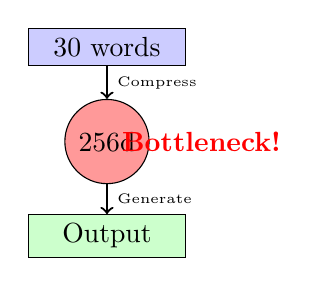
\begin{tikzpicture}[scale=0.6]
            \node[draw, rectangle, minimum width=2cm, fill=blue!20] (words) at (0,0) {30 words};

            \node[draw, circle, fill=red!40, minimum size=1cm] (bottle) at (0,-2) {256d};

            \node[draw, rectangle, minimum width=2cm, fill=green!20] (out) at (0,-4) {Output};

            \draw[->, thick] (words) -- (bottle) node[midway, right] {\tiny Compress};
            \draw[->, thick] (bottle) -- (out) node[midway, right] {\tiny Generate};

            \node at (2,-2) {\textcolor{red}{\textbf{Bottleneck!}}};
        \end{tikzpicture}
        \end{center}

        \textbf{Problem:}
        \begin{itemize}
            \item 30 words $\rightarrow$ 1 vector
            \item Information loss inevitable
            \item Same context for all outputs
        \end{itemize}

        \column{0.48\textwidth}
        \textbf{New Way (Selection):}

        \begin{center}
        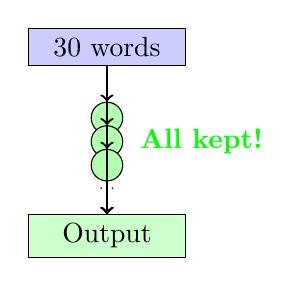
\begin{tikzpicture}[scale=0.6]
            \node[draw, rectangle, minimum width=2cm, fill=blue!20] (words) at (0,0) {30 words};

            \node[draw, circle, fill=green!30, minimum size=0.4cm] (s1) at (0,-1.5) {};
            \node[draw, circle, fill=green!30, minimum size=0.4cm] (s2) at (0,-2) {};
            \node[draw, circle, fill=green!30, minimum size=0.4cm] (s3) at (0,-2.5) {};
            \node at (0,-3) {\tiny ...};

            \node[draw, rectangle, minimum width=2cm, fill=green!20] (out) at (0,-4) {Output};

            \draw[->, thick] (words) -- (s1);
            \draw[->, thick] (words) -- (s2);
            \draw[->, thick] (words) -- (s3);

            \draw[->, thick] (s1) -- (out);
            \draw[->, thick] (s2) -- (out);
            \draw[->, thick] (s3) -- (out);

            \node at (2,-2) {\textcolor{green}{\textbf{All kept!}}};
        \end{tikzpicture}
        \end{center}

        \textbf{Solution:}
        \begin{itemize}
            \item Keep ALL encoder states
            \item Select relevant ones per output
            \item Different context each time
        \end{itemize}
    \end{columns}

    \vspace{0.5em}
    \textbf{Key Insight:} Don't throw away information, just focus on what matters!

    \vspace{0.5em}
    \textbf{Analogy:} Instead of summarizing a book, keep the full book and read relevant pages as needed.
\end{frame}

\begin{frame}[t]{Attention = Weighted Relevance (Zero Jargon)}
    \textbf{Breaking down ``attention'' into simple concepts:}

    \vspace{0.5em}
    \textbf{Setup:}
    \begin{itemize}
        \item 5 source words: [The, black, cat, sat, on]
        \item Generating French word ``chat'' (cat)
        \item Question: How relevant is each source word?
    \end{itemize}

    \vspace{0.5em}
    \begin{columns}[T]
        \column{0.5\textwidth}
        \textbf{Intuitive relevance scores:}

        \begin{center}
        \begin{tabular}{|l|c|c|}
            \hline
            \textbf{Word} & \textbf{Relevance} & \textbf{Why} \\
            \hline
            The & 5\% & Generic article \\
            black & 15\% & Describes cat \\
            cat & \textcolor{red}{70\%} & Direct match! \\
            sat & 5\% & Action, not noun \\
            on & 5\% & Preposition \\
            \hline
            \textbf{Total} & \textbf{100\%} & Must sum to 1 \\
            \hline
        \end{tabular}
        \end{center}

        \column{0.48\textwidth}
        \textbf{What these percentages do:}

        \vspace{0.5em}
        Context for ``chat'' = weighted average:

        \begin{align*}
            &= 0.05 \times h_{\text{The}}\\
            &+ 0.15 \times h_{\text{black}}\\
            &+ 0.70 \times h_{\text{cat}}\\
            &+ 0.05 \times h_{\text{sat}}\\
            &+ 0.05 \times h_{\text{on}}
        \end{align*}

        \vspace{0.5em}
        \textbf{Result:} Context is \textit{mostly} ``cat'' info, with a bit of everything else

        \vspace{0.5em}
        \highlight{These percentages ARE the attention weights!}
    \end{columns}
\end{frame}

\begin{frame}[fragile,t]{Why Dot Product Measures Relevance}
    \textbf{Geometric intuition (building from 2D):}

    \vspace{0.5em}
    \textbf{Question:} How does the network compute those relevance percentages?

    \vspace{0.5em}
    \begin{columns}[T]
        \column{0.5\textwidth}
        \textbf{Vectors as arrows in space:}

        \begin{center}
        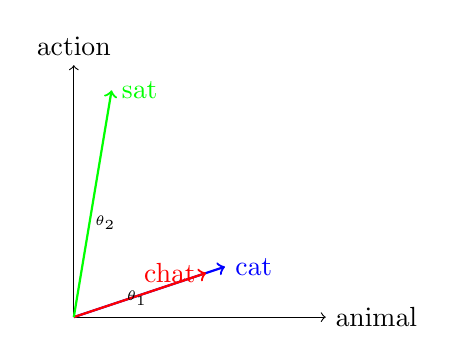
\begin{tikzpicture}[scale=0.8]
            \draw[->] (0,0) -- (4,0) node[right] {animal};
            \draw[->] (0,0) -- (0,4) node[above] {action};

            \draw[->, thick, blue] (0,0) -- (2.4,0.8) node[right] {cat};
            \draw[->, thick, red] (0,0) -- (2.1,0.7) node[left] {chat};
            \draw[->, thick, green] (0,0) -- (0.6,3.6) node[right] {sat};

            \node at (1,0.3) {\tiny $\theta_1$};
            \node at (0.5,1.5) {\tiny $\theta_2$};
        \end{tikzpicture}
        \end{center}

        \textbf{Properties of meaning:}
        \begin{itemize}
            \item ``cat'' = [0.8 animal, 0.2 action]
            \item ``chat'' = [0.7 animal, 0.2 action]
            \item ``sat'' = [0.2 animal, 0.9 action]
        \end{itemize}

        Similar meanings → similar directions!

        \column{0.48\textwidth}
        \textbf{Dot product measures alignment:}

        \vspace{0.5em}
        \textbf{cat · chat:}
        \begin{align*}
            &= (0.8 \times 0.7) + (0.2 \times 0.2)\\
            &= 0.56 + 0.04 = 0.60
        \end{align*}

        \textbf{cat · sat:}
        \begin{align*}
            &= (0.8 \times 0.2) + (0.2 \times 0.9)\\
            &= 0.16 + 0.18 = 0.34
        \end{align*}

        \vspace{0.5em}
        \textbf{Mathematical property:}
        \begin{itemize}
            \item Aligned vectors → High value
            \item Perpendicular → Zero
            \item Opposite → Negative
        \end{itemize}

        \vspace{0.5em}
        \highlight{Higher dot product = more relevant!}
    \end{columns}

    \vspace{0.5em}
    \textbf{In 256D:} Same principle, just more dimensions. Similar hidden states → high dot product.
\end{frame}

\begin{frame}[t]{The 3-Step Attention Mechanism}
    \textbf{Now we can understand the full algorithm:}

    \vspace{0.5em}
    \begin{columns}[T]
        \column{0.6\textwidth}
        \textbf{Step 1: Score (Measure Relevance)}

        For each encoder state, compute dot product with decoder state:

        \begin{align*}
            score_i &= h_{\text{decoder}} \cdot h_i^{\text{encoder}}
        \end{align*}

        \textbf{Why?} Dot product = alignment = relevance (from previous slide)

        \vspace{0.5em}
        \textbf{Step 2: Normalize (Make Probabilities)}

        Convert scores to weights that sum to 100\%:

        \begin{align*}
            \alpha_i &= \frac{\exp(score_i)}{\sum_j \exp(score_j)}
        \end{align*}

        \textbf{Why?} Need weights for weighted average

        \textbf{Tool:} Softmax function (ensures positive, sums to 1)

        \column{0.38\textwidth}
        \textbf{Step 3: Combine (Weighted Average)}

        Take weighted sum of encoder states:

        \begin{align*}
            context &= \sum_i \alpha_i \cdot h_i^{\text{encoder}}
        \end{align*}

        \textbf{Why?} Focus mostly on relevant, a bit on others

        \vspace{1em}
        \textbf{Example weights:}
        \begin{itemize}
            \item $\alpha_1$ (The) = 0.05
            \item $\alpha_2$ (black) = 0.15
            \item $\alpha_3$ (cat) = 0.70
            \item $\alpha_4$ (sat) = 0.05
            \item $\alpha_5$ (on) = 0.05
        \end{itemize}

        Context is mostly ``cat''!
    \end{columns}

    \vspace{0.5em}
    \textbf{Key Property:} Context is \textit{dynamic} - recomputed for each output word with different weights!

    \vspace{1em}
    \begin{checkpoint}[Understanding Attention]
    \textbf{Quick Check:} What are the 3 steps of attention?

    \vspace{0.3em}
    \textbf{Answer:}
    \begin{enumerate}
        \item \textbf{Score:} Dot product to measure relevance
        \item \textbf{Normalize:} Softmax to get weights (sum to 1)
        \item \textbf{Combine:} Weighted average of encoder states
    \end{enumerate}
    Result: Dynamic context focusing on relevant input words!
    \end{checkpoint}
\end{frame}

\begin{frame}[t]{Attention Calculation: Full Numerical Example}
    \textbf{Let's trace generating ``chat'' with actual numbers:}

    \vspace{0.5em}
    \textbf{Given:}
    \begin{itemize}
        \item Decoder state: $h_{\text{dec}} = [0.5, -0.2, 0.8]$
        \item Encoder states: $h_1 = [0.1, 0.2, 0.1]$ (The), $h_2 = [0.8, 0.1, 0.7]$ (cat), $h_3 = [0.2, 0.3, 0.2]$ (sat)
    \end{itemize}

    \vspace{0.5em}
    \begin{columns}[T]
        \column{0.6\textwidth}
        \textbf{Step 1: Compute scores (dot products)}

        \begin{align*}
            score_1 &= [0.5, -0.2, 0.8] \cdot [0.1, 0.2, 0.1]\\
            &= (0.5)(0.1) + (-0.2)(0.2) + (0.8)(0.1)\\
            &= 0.05 - 0.04 + 0.08 = 0.09\\
            \\
            score_2 &= [0.5, -0.2, 0.8] \cdot [0.8, 0.1, 0.7]\\
            &= (0.5)(0.8) + (-0.2)(0.1) + (0.8)(0.7)\\
            &= 0.40 - 0.02 + 0.56 = 0.94 \leftarrow \text{\textcolor{red}{Highest!}}\\
            \\
            score_3 &= [0.5, -0.2, 0.8] \cdot [0.2, 0.3, 0.2]\\
            &= (0.5)(0.2) + (-0.2)(0.3) + (0.8)(0.2)\\
            &= 0.10 - 0.06 + 0.16 = 0.20
        \end{align*}

        \column{0.38\textwidth}
        \textbf{Step 2: Softmax to weights}

        \begin{align*}
            \alpha_1 &= \frac{e^{0.09}}{e^{0.09} + e^{0.94} + e^{0.20}}\\
            &= \frac{1.09}{4.02} = 0.27\\
            \\
            \alpha_2 &= \frac{e^{0.94}}{4.02}\\
            &= \frac{2.56}{4.02} = 0.63\\
            \\
            \alpha_3 &= \frac{e^{0.20}}{4.02}\\
            &= \frac{1.22}{4.02} = 0.10
        \end{align*}

        \vspace{0.5em}
        \highlight{63\% attention on ``cat''!}

        \vspace{0.5em}
        \textbf{Step 3: Weighted context}

        \begin{align*}
            context &= 0.27 h_1\\
            &+ 0.63 h_2\\
            &+ 0.10 h_3
        \end{align*}
    \end{columns}

    \vspace{0.5em}
    \textbf{Interpretation:} Network learned to focus on ``cat'' when generating ``chat'' - correct alignment!
\end{frame}

\begin{frame}[t]{Visualizing Attention: The Alignment Matrix}
    \textbf{Attention weights reveal what the model is ``looking at'':}

    \vspace{0.5em}
    \begin{center}
    \includegraphics[width=0.65\textwidth]{../figures/week4_attention_heatmap.pdf}
    \end{center}

    \vspace{0.5em}
    \begin{columns}[T]
        \column{0.48\textwidth}
        \textbf{How to read this:}
        \begin{itemize}
            \item Rows = French output words
            \item Columns = English input words
            \item Brightness = attention weight
            \item Bright = high attention (looking here)
        \end{itemize}

        \column{0.48\textwidth}
        \textbf{Patterns discovered:}
        \begin{itemize}
            \item Diagonal: Similar word order
            \item Off-diagonal: Word reordering
            \item Multiple bright cells: Phrase translation
            \item \highlight{No supervision needed!}
        \end{itemize}
    \end{columns}

    \vspace{0.5em}
    \textbf{Key Insight:} This is interpretability - we can see the model's reasoning!
\end{frame}

\begin{frame}[t]{Why Attention Solves the Bottleneck}
    \textbf{Information capacity comparison:}

    \vspace{0.5em}
    \begin{columns}[T]
        \column{0.48\textwidth}
        \textbf{Without Attention:}

        \begin{itemize}
            \item 30 words compressed to 256d vector
            \item Capacity: 256 numbers (fixed)
            \item 30 words = ~3000 numbers needed
            \item \textcolor{red}{Overflow: 2744 numbers lost!}
            \item Same context for all outputs
        \end{itemize}

        \vspace{0.5em}
        \textbf{Information loss:}
        \begin{itemize}
            \item 91\% of information discarded
            \item Only high-level summary kept
            \item Details necessarily lost
        \end{itemize}

        \column{0.48\textwidth}
        \textbf{With Attention:}

        \begin{itemize}
            \item Keep all 30 encoder states
            \item Capacity: $30 \times 256 = 7680$ numbers
            \item All information preserved
            \item \textcolor{green}{Select relevant subset per output}
            \item Dynamic context each time
        \end{itemize}

        \vspace{0.5em}
        \textbf{Information preserved:}
        \begin{itemize}
            \item 100\% of information available
            \item Focus on relevant parts
            \item No forced compression
        \end{itemize}
    \end{columns}

    \vspace{0.5em}
    \begin{tcolorbox}[colback=green!10!white,colframe=green!75!black]
    \textbf{The Key Insight:} Dynamic selection beats static compression!

    Instead of ``compress everything to 256 numbers'', use ``keep everything, select as needed''
    \end{tcolorbox}
\end{frame}

\begin{frame}[t]{Attention Results: The Vindication}
    \textbf{Performance comparison validates the hypothesis:}

    \vspace{0.5em}
    \begin{center}
    \begin{tabular}{|l|c|c|c|}
        \hline
        \textbf{Sentence Length} & \textbf{No Attention} & \textbf{With Attention} & \textbf{Improvement} \\
        \hline
        5-10 words & 35.2 BLEU & 36.1 BLEU & +2.6\% \\
        10-20 words & 28.5 BLEU & 32.7 BLEU & +14.7\% \\
        20-30 words & 18.7 BLEU & 28.9 BLEU & +54.5\% \\
        30-40 words & 12.4 BLEU & 24.8 BLEU & +100\% \\
        40+ words & 8.1 BLEU & 24.3 BLEU & \textcolor{red}{+200\%} \\
        \hline
    \end{tabular}
    \end{center}

    \vspace{0.5em}
    \textbf{The pattern:}
    \begin{itemize}
        \item Short sentences: Small improvement (bottleneck wasn't the problem)
        \item Medium sentences: Moderate improvement (bottleneck starts to matter)
        \item Long sentences: \highlight{Massive improvement} (bottleneck was killing performance)
    \end{itemize}

    \vspace{0.5em}
    \begin{tcolorbox}[colback=blue!10!white,colframe=blue!75!black]
    \textbf{Validation:} Attention solves exactly the problem we diagnosed!

    Improvement is largest where bottleneck hurt most (long sentences).
    \end{tcolorbox}

    \vspace{0.5em}
    \textbf{Historical Impact:} This 2015 paper (Bahdanau et al.) launched the attention revolution in NLP.
\end{frame}

\begin{frame}[fragile,t]{Implementing Attention (Surprisingly Simple)}
    \textbf{The complete mechanism in code:}

    \vspace{0.5em}
    \begin{columns}[T]
        \column{0.55\textwidth}
        \begin{lstlisting}[language=Python]
def attention(decoder_state, encoder_states):
    """
    decoder_state: [256] - current decoder hidden state
    encoder_states: [seq_len, 256] - all encoder states
    Returns: context [256], attention_weights [seq_len]
    """
    scores = []

    for enc_state in encoder_states:
        score = dot(decoder_state, enc_state)
        scores.append(score)

    scores = array(scores)

    exp_scores = exp(scores - max(scores))
    attention_weights = exp_scores / sum(exp_scores)

    context = zeros(256)
    for i, enc_state in enumerate(encoder_states):
        context += attention_weights[i] * enc_state

    return context, attention_weights
        \end{lstlisting}

        \column{0.43\textwidth}
        \textbf{Three operations:}

        \begin{enumerate}
            \item \textbf{Lines 9-11:} Dot products\\(relevance scores)
            \item \textbf{Lines 15-16:} Softmax\\(probabilities)
            \item \textbf{Lines 18-20:} Weighted sum\\(dynamic context)
        \end{enumerate}

        \vspace{1em}
        \textbf{That's it!}

        Just 3 operations:
        \begin{itemize}
            \item Dot product (similarity)
            \item Softmax (normalize)
            \item Weighted sum (combine)
        \end{itemize}

        \vspace{0.5em}
        \textbf{Key difference:}

        Context recomputed EVERY step with different weights!
    \end{columns}

    \vspace{0.5em}
    \textbf{Checkpoint:} Can you trace what happens when decoder generates ``chat'' with input ``The cat sat''?
\end{frame}

\section{Act 4: Synthesis and Impact}

\begin{frame}[t]{The Three Key Ideas Combined}
    \textbf{Unified architecture diagram:}

    \vspace{0.5em}
    \begin{center}
    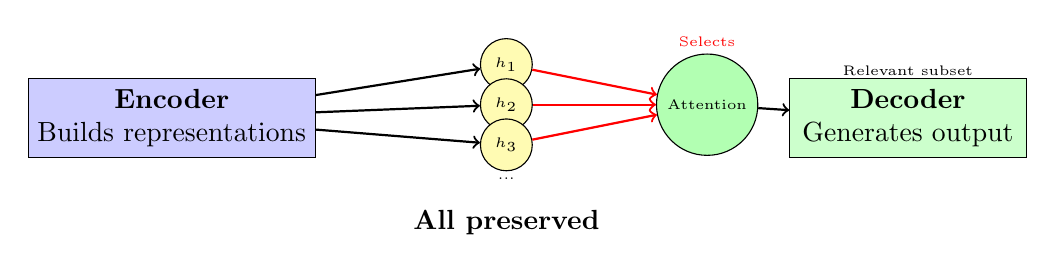
\begin{tikzpicture}[scale=0.85]
        \node[draw, rectangle, minimum width=3cm, minimum height=1cm, fill=blue!20, align=center] (input) at (0,0) {\textbf{Encoder}\\Builds representations};

        \node[draw, circle, fill=yellow!30, minimum size=0.5cm] (h1) at (5,0.8) {\tiny $h_1$};
        \node[draw, circle, fill=yellow!30, minimum size=0.5cm] (h2) at (5,0.2) {\tiny $h_2$};
        \node[draw, circle, fill=yellow!30, minimum size=0.5cm] (h3) at (5,-0.4) {\tiny $h_3$};
        \node at (5,-0.9) {\tiny ...};
        \node[below of=h2, node distance=1.5cm] {\textbf{All preserved}};

        \node[draw, circle, fill=green!30, minimum size=0.8cm, align=center] (attn) at (8,0.2) {\tiny Attention};

        \node[draw, rectangle, minimum width=3cm, minimum height=1cm, fill=green!20, align=center] (output) at (11,0) {\textbf{Decoder}\\Generates output};

        \draw[->, thick] (input) -- (h1);
        \draw[->, thick] (input) -- (h2);
        \draw[->, thick] (input) -- (h3);

        \draw[->, thick, red] (h1) -- (attn);
        \draw[->, thick, red] (h2) -- (attn);
        \draw[->, thick, red] (h3) -- (attn);
        \node[above of=attn, node distance=0.8cm, text=red] {\tiny Selects};

        \draw[->, thick] (attn) -- (output);
        \node[above of=output, node distance=0.6cm] {\tiny Relevant subset};
    \end{tikzpicture}
    \end{center}

    \vspace{0.5em}
    \textbf{The three innovations:}

    \begin{enumerate}
        \item \textbf{Two-stage architecture:} Separate reading (encoder) from writing (decoder)
        \begin{itemize}
            \item Handles variable-length input and output
            \item Mimics human translation process
        \end{itemize}

        \item \textbf{Sequence-to-sequence:} No fixed input/output size
        \begin{itemize}
            \item 3 words in → 2 words out (possible!)
            \item 100 words in → 50 words out (possible!)
        \end{itemize}

        \item \textbf{Attention mechanism:} Dynamic selection over static compression
        \begin{itemize}
            \item Solves information bottleneck
            \item Provides interpretability
            \item Enables long-sentence translation
        \end{itemize}
    \end{enumerate}
\end{frame}

\begin{frame}[t]{What We Learned (Conceptual Insights)}
    \textbf{Beyond seq2seq - general lessons:}

    \vspace{0.5em}
    \begin{enumerate}
        \item \textbf{Compression Trade-off:} Information capacity fundamentally limits performance
        \begin{itemize}
            \item Can't fit arbitrary information into fixed size
            \item Longer inputs → worse compression → lost details
            \item Quantifiable: compression ratio predicts quality degradation
        \end{itemize}

        \vspace{0.5em}
        \item \textbf{Selection > Compression:} For complex tasks, keep everything and select
        \begin{itemize}
            \item Don't throw away information prematurely
            \item Dynamic selection more flexible than static summary
            \item ``Soft'' selection (weighted average) enables gradient flow
        \end{itemize}

        \vspace{0.5em}
        \item \textbf{Learned Alignment:} Network discovers correspondences without supervision
        \begin{itemize}
            \item Attention weights show word alignments
            \item Model learns which source words matter for each output
            \item Interpretable - we can visualize reasoning
        \end{itemize}

        \vspace{0.5em}
        \item \textbf{Differentiable Operations:} All steps trainable via backpropagation
        \begin{itemize}
            \item Score, softmax, weighted sum all have gradients
            \item End-to-end learning of entire system
            \item No hand-crafted alignment rules needed
        \end{itemize}
    \end{enumerate}
\end{frame}

\begin{frame}[t]{Beyond Translation: 2024 Applications}
    \textbf{The attention explosion across AI:}

    \vspace{0.5em}
    \begin{columns}[T]
        \column{0.48\textwidth}
        \textbf{Language (Original):}
        \begin{itemize}
            \item Machine translation (133 languages)
            \item Text summarization
            \item Question answering
            \item Dialogue systems
        \end{itemize}

        \vspace{0.5em}
        \textbf{Vision:}
        \begin{itemize}
            \item Image captioning (attend to regions)
            \item Visual question answering
            \item Object detection
            \item Image generation (DALL-E)
        \end{itemize}

        \column{0.48\textwidth}
        \textbf{Speech:}
        \begin{itemize}
            \item Speech recognition (attend to audio frames)
            \item Speech synthesis
            \item Real-time translation
        \end{itemize}

        \vspace{0.5em}
        \textbf{Modern AI:}
        \begin{itemize}
            \item \textbf{Transformers:} Pure attention (Week 5!)
            \item GPT-4, Claude, Gemini
            \item Multimodal models (CLIP)
            \item All modern LLMs use attention
        \end{itemize}
    \end{columns}

    \vspace{0.5em}
    \textbf{Historical timeline:}
    \begin{itemize}
        \item 2014: Seq2seq (encoder-decoder)
        \item 2015: Attention mechanism (this lecture!)
        \item 2017: Transformers (``Attention is All You Need'')
        \item 2018+: BERT, GPT, current AI revolution
    \end{itemize}

    \vspace{0.5em}
    \highlight{Attention is the foundation of all modern AI systems!}
\end{frame}

\begin{frame}[t]{Summary: The Complete Compression Journey}
    \textbf{What you now understand from first principles:}

    \vspace{0.5em}
    \begin{enumerate}
        \item \textbf{Why embeddings:} Computers need numbers, embeddings give numerical meaning
        \begin{itemize}
            \item Similar words → similar vectors
            \item From bytes to meaning
        \end{itemize}

        \item \textbf{Why hidden states:} Capture evolving understanding as we read
        \begin{itemize}
            \item Accumulates meaning word-by-word
            \item Final state = complete sentence understanding
        \end{itemize}

        \item \textbf{Why encoder-decoder:} Separate reading from writing
        \begin{itemize}
            \item Handles variable lengths
            \item Mimics human translation
        \end{itemize}

        \item \textbf{Why context vectors:} Compress meaning, but creates bottleneck
        \begin{itemize}
            \item Fixed size for any input
            \item Information overflow gets lost
        \end{itemize}

        \item \textbf{Why attention:} Solve bottleneck by keeping all states and selecting
        \begin{itemize}
            \item Dynamic selection beats compression
            \item 200\% improvement on long sentences
        \end{itemize}

        \item \textbf{Why dot product:} Geometric measure of relevance (vector alignment)
        \begin{itemize}
            \item Similar directions → high value
            \item Differentiable for training
        \end{itemize}
    \end{enumerate}

    \vspace{0.5em}
    \textbf{Next week:} Remove encoder/decoder RNNs, use ONLY attention → Transformers!
\end{frame}

% ==================== APPENDIX: MATHEMATICAL DETAILS ====================

\appendix

% Appendix Slide 1: Seq2seq Mathematics
\begin{frame}{Appendix A: Seq2Seq Mathematics - Complete Equations}
    \begin{columns}[T]
        \begin{column}{0.48\textwidth}
            \textbf{Encoder (RNN Processing):}

            \vspace{0.5em}
            At each time step $t = 1, 2, \ldots, T_x$:

            \vspace{0.3em}
            \textbf{1. Embedding lookup:}
            \[
            x_t = \text{Embed}(w_t) \in \mathbb{R}^{d_{\text{emb}}}
            \]

            \vspace{0.3em}
            \textbf{2. Encoder hidden state:}
            \[
            h_t^{\text{enc}} = \text{RNN}_{\text{enc}}(x_t, h_{t-1}^{\text{enc}})
            \]

            Explicitly:
            \[
            h_t^{\text{enc}} = \tanh(W_x x_t + W_h h_{t-1}^{\text{enc}} + b_h)
            \]

            where $h_t^{\text{enc}} \in \mathbb{R}^{d_h}$ (typically 256-512d)

            \vspace{0.5em}
            \textbf{3. Context vector:}
            \[
            c = h_{T_x}^{\text{enc}}
            \]

            (Final encoder state = compressed meaning)

            \vspace{0.5em}
            \textbf{Encoder Dimensions:}
            \begin{itemize}
                \item Vocabulary: $|V| = 10,000$ to $50,000$
                \item Embedding: $d_{\text{emb}} = 128$ to $512$
                \item Hidden: $d_h = 256$ to $1024$
            \end{itemize}
        \end{column}

        \begin{column}{0.48\textwidth}
            \textbf{Decoder (Generation):}

            \vspace{0.5em}
            Initialize: $s_0 = c$ (context from encoder)

            \vspace{0.5em}
            At each generation step $t = 1, 2, \ldots, T_y$:

            \vspace{0.3em}
            \textbf{1. Decoder hidden state:}
            \[
            s_t = \text{RNN}_{\text{dec}}(y_{t-1}, s_{t-1}, c)
            \]

            Explicitly:
            \[
            s_t = \tanh(W_y y_{t-1} + W_s s_{t-1} + W_c c + b_s)
            \]

            \vspace{0.3em}
            \textbf{2. Output distribution:}
            \[
            P(y_t \given y_{<t}, x) = \text{softmax}(W_o s_t + b_o)
            \]

            \vspace{0.3em}
            \textbf{3. Teacher forcing (training):}
            \[
            y_{t-1} = y_{t-1}^* \quad \text{(use true previous word)}
            \]

            \vspace{0.3em}
            \textbf{4. Loss function:}
            \[
            L = -\sum_{t=1}^{T_y} \log P(y_t^* \given y_{<t}, x)
            \]

            \vspace{0.5em}
            \textbf{Training:}
            \begin{itemize}
                \item Backpropagation through time (BPTT)
                \item Gradient clipping (prevent explosion)
                \item Teacher forcing ratio: 0.5-1.0
            \end{itemize}
        \end{column}
    \end{columns}

    \bottomnote{Context vector $c$ is the bottleneck - fixed 256-512d for ANY input length!}
\end{frame}

% Appendix Slide 2: Attention Mathematical Derivation
\begin{frame}{Appendix B: Attention Mechanism - Mathematical Derivation}
    \begin{columns}[T]
        \begin{column}{0.48\textwidth}
            \textbf{The Attention Computation:}

            \vspace{0.5em}
            Given encoder hidden states $\{h_1^{\text{enc}}, \ldots, h_{T_x}^{\text{enc}}\}$ and decoder state $s_t$:

            \vspace{0.5em}
            \textbf{Step 1: Alignment Scores}

            Compute relevance of each encoder state:
            \[
            e_{t,i} = \text{score}(s_t, h_i^{\text{enc}})
            \]

            \textbf{Common scoring functions:}

            \vspace{0.3em}
            \textit{Dot product} (Luong attention):
            \[
            e_{t,i} = s_t^T h_i^{\text{enc}}
            \]

            \vspace{0.3em}
            \textit{Additive} (Bahdanau attention):
            \[
            e_{t,i} = v^T \tanh(W_s s_t + W_h h_i^{\text{enc}})
            \]

            \vspace{0.5em}
            \textbf{Step 2: Attention Weights}

            Normalize scores to probabilities:
            \[
            \alpha_{t,i} = \frac{\exp(e_{t,i})}{\sum_{j=1}^{T_x} \exp(e_{t,j})}
            \]

            Properties:
            \begin{itemize}
                \item $\alpha_{t,i} \geq 0$ (non-negative)
                \item $\sum_{i=1}^{T_x} \alpha_{t,i} = 1$ (sum to 1)
            \end{itemize}
        \end{column}

        \begin{column}{0.48\textwidth}
            \textbf{Step 3: Context Vector}

            Weighted sum of encoder states:
            \[
            c_t = \sum_{i=1}^{T_x} \alpha_{t,i} h_i^{\text{enc}}
            \]

            \textbf{Key property:} Context $c_t$ is DYNAMIC - recomputed at each decoder step with different weights!

            \vspace{0.5em}
            \textbf{Modified Decoder with Attention:}

            \[
            s_t = \text{RNN}_{\text{dec}}(y_{t-1}, s_{t-1}, c_t)
            \]

            \vspace{0.5em}
            \textbf{Why Softmax?}

            \begin{enumerate}
                \item \textbf{Normalization:} Ensures weights sum to 1
                \item \textbf{Differentiability:} Smooth function for backprop
                \item \textbf{Sparsity:} Exponentiation amplifies differences:
                \[
                e_1 = 0.9, e_2 = 0.1 \rightarrow \alpha_1 = 0.64, \alpha_2 = 0.36
                \]
                \[
                e_1 = 5.0, e_2 = 1.0 \rightarrow \alpha_1 = 0.98, \alpha_2 = 0.02
                \]
            \end{enumerate}

            \vspace{0.5em}
            \textbf{Computational Complexity:}
            \begin{itemize}
                \item Scores: $O(T_x \cdot d_h)$ per decoder step
                \item Total: $O(T_x \cdot T_y \cdot d_h)$
                \item Quadratic in sequence length!
            \end{itemize}

            (Transformers address this - Week 5!)
        \end{column}
    \end{columns}

    \bottomnote{Attention creates dynamic, interpretable alignment between source and target sequences}
\end{frame}

\end{document}